\hsection{Fixed:~Transitive Dependency factored out into own Table}%
\FloatBarrier%
%
\begin{figure}%
\centering%
%
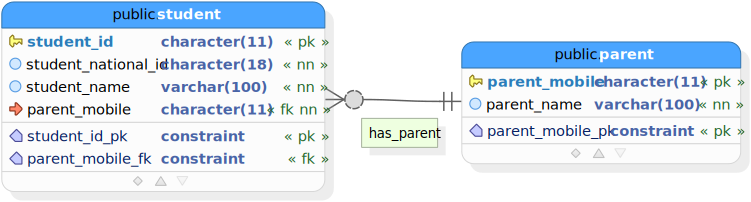
\includegraphics[width=0.875\linewidth]{\currentDir/studentFixed3nf}%
%
\caption{Two tables which store data about students and their parents and which, different from \cref{fig:studentViolation3nf}, do not violate the \pgls{3NF}.}%
\label{fig:studentFixed3nf}%
\end{figure}%
%
\gitExecSQLraw{}{}{normalization/3nf/student/fixed/generated_sql}{01_fixed_database_2001.sql}{}{}{}
%
\gitLoadAndExecSQL{3nf:student:fixed:03_public_student_table_5071}{}{normalization/3nf/student/fixed/generated_sql}{03_public_student_table_5071.sql}{fixed}{}{}%
\listingSQL{3nf:student:fixed:03_public_student_table_5071}{%
he generated \sql\ code for creating the table \sqlil{student}.}%
%
\gitLoadAndExecSQL{3nf:student:fixed:04_public_parent_table_5077}{}{normalization/3nf/student/fixed/generated_sql}{04_public_parent_table_5077.sql}{fixed}{}{}%
\listingSQL{3nf:student:fixed:04_public_parent_table_5077}{%
The generated \sql\ code for creating the table \sqlil{parent}.}%
%
\gitLoadAndExecSQL{3nf:student:fixed:05_public_student_parent_mobile_fk_constraint_5081}{}{normalization/3nf/student/fixed/generated_sql}{05_public_student_parent_mobile_fk_constraint_5081.sql}{fixed}{}{}%
\listingSQL{3nf:student:fixed:05_public_student_parent_mobile_fk_constraint_5081}{%
We add the foreign key constraint to table~\sqlil{student}.}%
%
\gitLoadAndExecSQL{3nf:student:fixed:insert}{}{normalization/3nf/student/fixed}{insert.sql}{fixed}{}{}%
\listingSQL{3nf:student:fixed:insert}{%
Inserting some data into the tables~\sqlil{parent} and~\sqlil{student}.}%
%
\gitLoadAndExecSQL{3nf:student:fixed:select}{}{normalization/3nf/student/fixed}{select.sql}{fixed}{}{}%
\listingSQLandOutput{3nf:student:fixed:select}{%
If we want to get the names of the parents of the students, we now need an~\sqlilIdx{INNER JOIN}.%
}{}%
%
\gitLoadAndExecSQL{3nf:student:fixed:update}{}{normalization/3nf/student/fixed}{update.sql}{fixed}{}{}%
\listingSQLandOutput{3nf:student:fixed:update}{%
We noticed that the name of the father of Mr.~Bibbo, Mr.~Bibotto, and Ms.~Bibboba is actually Mr.~B{\"o}dd{\"o}, not Mr.~Boddo. %
Since we now observe the \pgls{3NF}, we need to touch only a single records to change this.%
}{}%
%
\gitExecSQLraw{}{}{normalization/3nf/student/fixed}{cleanup.sql}{}{}{}%
%
%
Let us fix this problem.
We need to bring the data into the \pgls{3NF}.
For this, we need to remove the transitive functional dependency \funcDepb{\sqlil{student_id}}{\funcDepb{\sqlil{parent_mobile}}{\sqlil{parent_name}}}.
This dependency is problematic because \sqlil{parent_mobile} was no key of table \sqlil{student}, but \sqlil{parent_name} was determined by \sqlil{parent_mobile}.
As long as these three columns are in the same table, the \pgls{3NF} will always be violated.
So they need to be separated into different tables.

In \cref{fig:studentFixed3nf} we illustrate a logical model that no longer violates the \pgls{3NF}.
Different from our original sketch in \cref{fig:studentViolation3nf}, we use two tables instead of one.
The name of the parent depends on their mobile phone number.
So we remove this data from the original \sqlil{student}~table and put it into a table~\sqlil{parent}.
This table has the primary key~\sqlil{parent_mobile}.
This value is unique and identifies a parent.
The second column of this table~\sqlil{name}, which obviously depends on that primary key.

The modified table~\sqlil{student} now uses the attribute~\sqlil{parent_mobile} as foreign key.
It must be \sqlilIdx{NOT NULL}, meaning that each row in table~\sqlil{student} is linked to one~(and exactly one) row in table~\sqlil{parent}.
We now no longer store the name of the parent in the \sqlil{student}~table.

Both tables observe the \pgls{1NF}, as there are neither composite attributes nor repeated groups.
Both also observe the \pgls{2NF}, because there is no compound key and, hence, it is not possible that an attribute could depend on a part of such a key only.
They also both observe the \pgls{3NF}, because there is no transitive functional dependency.

As a side note, observe that we could also have used a surrogate primary key here for the table~\sqlil{parent}, which would probably be the better solution.
This would have allowed us to later change the mobile phone number of a parent, without the need to touch the table~\sqlil{student}.
Changing the structure for this would be a nice exercise for the keen reader.

Let us look at this system in action.
We first create the table~\sqlil{student} by executing the script given in \cref{lst:3nf:student:fixed:03_public_student_table_5071}.
It retained the three columns \sqlil{student_id}, \sqlil{student_name}, and \sqlil{parent_mobile}.
But it lost the column \sqlil{parent_name}.
The primary key is still \sqlil{student_id}.
The column \pythonil{parent_mobile} will become a foreign key to the table for the parent records.

\Cref{lst:3nf:student:fixed:04_public_parent_table_5077} then creates the new table~\sqlil{parent} for exactly these parent records.
This table has only two columns:
the primary key \pythonil{parent_mobile}, which is still a string of the fixed length~11, and the parent name.

Script \cref{lst:3nf:student:fixed:05_public_student_parent_mobile_fk_constraint_5081}, adds the foreign key constraint to table~\sqlil{student}.
This step is what actually turns \pythonil{parent_mobile} into a foreign key of table~\sqlil{student}.
This constraint enforces that each row in table~\sqlil{student} is related to exactly one row in table~\sqlil{parent}.

We can now insert data into this new \db\ structure.
In \cref{lst:3nf:student:violation:insert}, we begin by storing the two parent records into the table~\sqlil{parent}.
The mobile phone numbers and names of Ms.~Balla, the mom of Mr.~Bebbo, as well as Mr.~B{\"o}dd{\"o}, the dad of the other three students are stored.
Like last time, our data entry specialist did, at first, not know how to write the the fancy~\keys{\"o} in name Mr.~B{\"o}dd{\"o} and resorted to just call him~Mr.~Boddo.
Then we insert four student records for Mr.~Bibbo, Mr.~Bebbo, Mr.~Bibboto, and Ms.~Bibboba.
Here, we do not provide their parent's names anymore.
Only their mobile phone numbers, linking to table~\sqlil{parent}, are needed.

At first glance, this new structure looks more complicated.
We now have two tables instead of one.
If we want to know the names of the parents of the students, a simple~\sqlilIdx{SELECT} will no longer be enough.
Instead, we need to merge the data from two tables by using an~\sqlilIdx{INNER JOIN}, as shown in \cref{lst:3nf:student:fixed:select}.

One could argue that the advantage is the reduced redundancy:
The name of each parent is entered once and only one.
Then again, you may argue that in this simple example, this advantage is more or less offset by the fact that we need to enter their mobile phone numbers in both tables.
This only matters in this example because the example is a minimal corner case.
We only extracted a single column.
Often, there could be many columns.
Imagine that we also stored the parent address and ID number and so on.
Generally, the redundancy reduction is a good argument.

The usefulness of the new design becomes clearer when we change data.
Like in our original example, a few days after originally entering the data, our data entry specialist found a solution on how to enter the letter~\keys{\"o}.
In order to fix the data, they created the script \cref{lst:3nf:student:violation:update}.
The \sqlilIdx{UPDATE} command is now applied to table~\sqlil{parent}.
It only touches a single row, as you can see by the result of the \sqlilIdx{RETURNING} statement.
In the same script, we use another \sqlilIdx{SELECT} to check whether the parent names of Mr.~Bibbo, Mr.~Bibboto, and Ms.~Bibboba have changed.
And indeed, they have.
The update anomaly has disappeared.
%
\FloatBarrier%
\endhsection%
%
